\documentclass[12pt]{article}
%
%
% Retirez le caractere "%" au debut de la ligne ci-dessous si votre
% editeur de texte utilise des caracteres accentues
% \usepackage[latin1]{inputenc}

%
% Retirez le caractere "%" au debut des lignes ci-dessous si vous
% utiisez les symboles et macros de l'AMS
 \usepackage{amsmath}
% \usepackage{amsfonts}
%
%
\usepackage[left=2.5cm,right=2.5cm,top=2.5cm,bottom=2.5cm]{geometry}
\setlength{\parskip}{6pt}
\usepackage{graphicx}
\usepackage{xcolor} % ARO modified color to xcolor

% Nouvelles commandes pour ajouter nos commentaires en couleur

\newcommand{\tdo}{\textcolor{red}{\textbf{TO DO}}}

% ARO added
\usepackage[french,english]{babel}


\usepackage{ragged2e} % Provides \justify command
\usepackage{booktabs}
\usepackage[T1]{fontenc}


\begin{document}

\selectlanguage{french}
\justify % Justify the text


\begin{enumerate}
  \item \textbf{Qu'est-ce que l'inégalité triangulaire ?} 
  
  $|x + y| < |x| + |y|$

  \item \textbf{En quelle année a lieu la bataille de Marignan et quelles forces s'y opposent ?}
  
  En 1515, elle oppose les Français et leurs alliés vénitiens aux mercenaires suisses qui défendent le duché de Milan

  \item \textbf{Que vaut $cos(\pi / 6)$ ?}
  
  $\sqrt(3/2)$

  \item \textbf{En quelle année l'Algérie devient-elle indépendante ?}
  
  1962

  \item \textbf{Qu'est-ce que le premier Principe de la thermodynamique ?}
  
  Au cours d'une transformation quelconque d'un système fermé, la variation de son énergie est égale à la quantité d'énergie échangée avec le milieu extérieur, par transfert thermique (chaleur) et transfert mécanique (travail). 
  
  \item \textbf{Combien de temps dure la préhistoire ?}
  
  Plus de 3 millions d'années
  
  \item \textbf{Quelle est la 3ème loi de Newton ?}
  
  La troisième loi de Newton est le principe de l'action et de la réaction. Si un corps A exerce une force sur un corps B, alors B exerce sur A une force d'égale intensité, de même direction et de sens opposé.
  
  \item \textbf{Quel texte est promulgué par Henri IV afin de mettre fin aux guerres de religion (et plus particulièrement la huitième) qui ravagent le royaume de France et en quelle année l'est-il ?}
  
  Edit de Nantes, 1598

  \item \textbf{Où peut-on trouver des mitochondries et quel est leur rôle ?}
  
  Dans les cellules, elles leur fournissent de l'énergie.
  
  \item \textbf{Quel est le théoreme de Bernoulli ?}
  
  La quantité de Bernoulli se conserve le long de chaque chemin tangent au champ des vitesses. En d'autres termes, sur une ligne de courant
  
  \item \textbf{Quelle bataille oppose les Francs et Aquitains, menés par Charles Martel d'une part à l'armé Omeyyade menée par Abd al Rahman, et en quelle année a-t-elle lieu ?}
  
  Bataille de Poitiers, 732
  
  \item \textbf{Quelle est la différence entre un alcane, un alcène et un alcyne ?}
  
  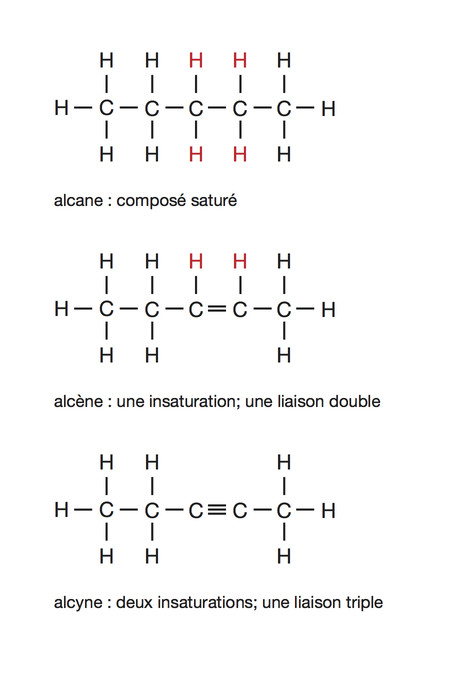
\includegraphics[height=10cm,width=9cm]{alcane.png}
  
  \item \textbf{En quelle année est adopté le suffrage universel en France ?}
  
  1848
  
  \item \textbf{Qu'est-ce que la loi de Poisson ?}
  
  La loi de Poisson est une loi de probabilité discrète qui décrit le comportement du nombre d'événements se produisant dans un intervalle de temps fixé, si ces événements se produisent avec une fréquence moyenne ou espérance connue, et indépendamment du temps écoulé depuis l'événement précédent.
  
  \item \textbf{De combien de plaques tectoniques est composée la surface de la terre (+/- 2) ?}
  
  12
  
  \item \textbf{Qu'est-ce que le théoreme de Malus en optique ?}
  
  La surface d'onde est perpendiculaire au rayon lumineux en chacun de ses points.
  
  \item \textbf{Combien de pays compte l'OCDE ? En citer 5 qui ne sont pas membres permanents de conseil de sécurité de l'ONU }
  
  20 pays.
  
  Réponses possibles : Austria, Belgium, Canada, Denmark, West Germany, Greece, Iceland, Ireland, Italy, Luxembourg, Netherlands, Norway, Portugal, Spain, Sweden, Switzerland, Turkey.
  
  \item \textbf{Qu'est-ce qu'une transformation adiabatique ?}
  
  C'est une transformation qui ne produit pas d'échange de chaleur avec le milieu extérieur.
  
  \item \textbf{Quel pourcentage de la surface de la terre représentent les continents ?}
  
  30\%

  \item \textbf{Citer le nom de 3 des 4 caïds de notre classe de 3ème ?}
  
  LG, BZ, TT
  
  \item \textbf{Quelle est la transformée de Laplace de $e^{at}$ ?}
  
  $\frac{1}{z-a}$
  
  \item \textbf{En quelle année naît la Vème république en France ?}
  
  1958
  
  \item \textbf{Quel est le personnage principal des \textit{fausses confidences} de Marivaux ?}
  
  Dorante
  
  \item \textbf{Donner la loi de Fourier appliquée a une ailette en transferts thermiques ?}
  
  $\Phi = -\lambda * S dT dx$
  
  \item \textbf{Donner le nom de trois listes BDE qui ont gagné leur campagne ?}
  
  Police Acadmey, Bananalist

  \item \textbf{Réciter la première déclinaison en latin ?}
  
  Singulier : Rosa, rosa, rosam, rosae, rosae, rosa.

  Pluriel : Rosae, rosae, rosas, rosarum, rosis, rosis. 
  
  \item \textbf{Quelle monnaie commune européenne précède l'EURO ?}
  
  L'ECU (European Currency Unit)
  
  \item \textbf{Donner le nom de trois personnes appartenant au ski club à Centrale ?}
  
  Dimitri Pleple, Charles Puybasset, Antoine Walckanear

  \item \textbf{Réciter le premier vers de l'hymne national Sud-Africain ?}
  
  Nkosi Sikelel' iAfrika
  
  \item \textbf{Qu’est-ce que le problème de Cauchy ?}
  
  En analyse, un problème de Cauchy est un problème constitué d'une équation différentielle dont on recherche une solution vérifiant une certaine condition initiale. 
  
  \item \textbf{Nom du président de CeC a Centrale ?}
  
  Clement Hammel.

  \item \textbf{Citer les 8 présidents de la Vème République en France ?}
  
  Charles de Gaulle, Georges Pompidou, VGE, Mitterand, Chirac, Sarkozy, Hollande, Macron.

  \item \textbf{En quelle année l'équipe d'Angleterre de Football a-t-elle remporté la Coupe du Monde ?}
  
  1966
  
  \item \textbf{Quelle est la valeur de la constante d'Avogadro ? A quoi sert-elle ? ?}
  
  C'est le nombre d'entités (atomes, molécules, ions ou particules) qui se trouvent dans une mole de matière. Il est de $6 \times 10^{23}$

  \item \textbf{Qu'est-ce que l'équation de Schrodinger en physique quantique ?}
  
  $2m \phi''(x) + qV (x)\phi(x) = E\phi(x)$
  
  \item \textbf{Quelle sont les 5 premières universités du classement de Shanghaï en 2024 ?}
  
  Harvard, Stanford, MIT, Cambridge, Berkeley
  
  \item \textbf{Toujours sur le classement de Shanghaï, quelle est l'université française la mieux classée et en quelle position est-elle ?}
  
  Paris Saclay, 15ème
   
  \item \textbf{Comment dit-on maître au datif singulier en latin ?}
  
  Domino.
  
  \item \textbf{Quel est l'élément déclencheur de la première guerre mondiale ?}
  
  L'assassinat de l'archiduc Franz Ferdinand d'Autriche à Sarajevo.

  \item \textbf{Comment dit-on grand-père en espagnol ?}
  
  Abuelo.

\end{enumerate}



\end{document}